%   MSc Business Analytics Dissertation
%
%   Title:     Aaa Bbbbbbb Cccccccccc
%   Author(s): Xxxxxx Xxxxxxxxx and Yyy Yyyyyyyyy
%
%   Appendix 1: long tables
%
%   Change Control:
%   When     Who   Ver  What
%   -------  ----  ---  --------------------------------------------------------------
%   11Feb11  AB    0.1  Begun 
%

\chapter{Feature Descriptions}\label{C.Appendix1}
{The following table contains long form descriptions for some of the main variables used in this study. This table is reproduced from the work of \cite{moldovan2015learning}. }
\iffalse
\begin{figure}[h!]
\centering
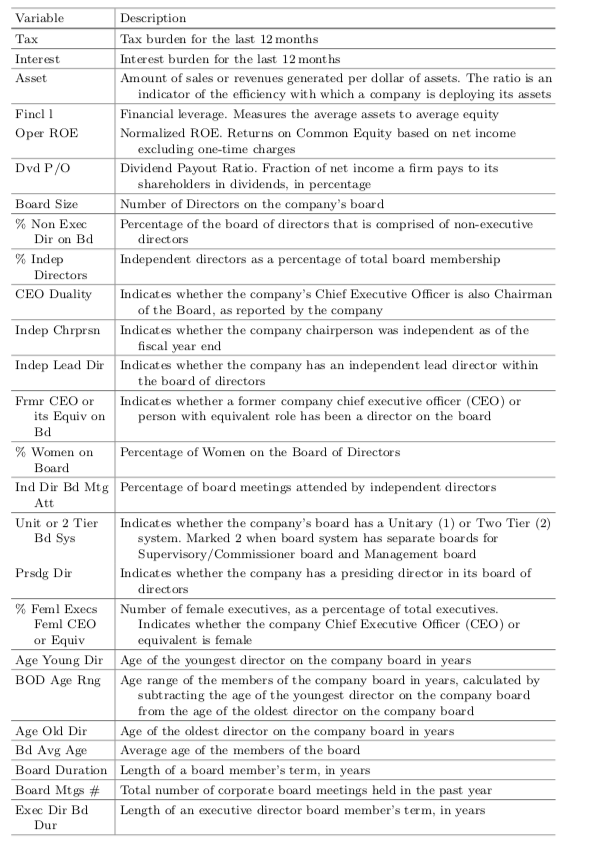
\includegraphics[scale=0.65]{images/var_desc.png}
\end{figure}
\fi

\begin{table}[h!]
\scalebox{0.8}{
\begin{tabular}{ |p{5cm}|p{12cm}| }
 \hline
 {\bf Variable} & {\bf Description}  \\
 \hline
Tax &Tax burden for the last 12 months \\
\rowcolor{gray}Interest&Interest burden for the last 12 months \\
Asset&Amount of sales or revenues generated per dollar of assets. The ratio is an indicator of the efficiency with which a company is deploying its assets \\
\rowcolor{gray}Fincl&Financial leverage. Measures the average assets to average equity \\
Oper ROE&Normalized ROE. Returns on Common Equity based on net income excluding one-time charges \\
\rowcolor{gray}Dvd P/O&Dividend Payout Ratio. Fraction of net income a firm pays to its shareholders in dividends, in percentage \\
Board Size&Number of Directors on the company?s board \\
\rowcolor{gray}\% Non Exec Dir on Bd &Percentage of the board of directors that is comprised of non-executive directors \\
\% Indep Directors &Independent directors as a percentage of total board membership \\
\rowcolor{gray}CEO Duality &Indicates whether the company?s Chief Executive Officer is also Chairman of the Board, as reported by the company \\
Indep Chrprsn&Indicates whether the company chairperson was independent as of the fiscal year end \\
\rowcolor{gray}Indep Lead Dir&Indicates whether the company has an independent lead director within the board of directors \\
Frmr CEO or its Equiv on Bd&Indicates whether a former company chief executive officer (CEO) or person with equivalent role has been a director on the board \\
\rowcolor{gray}\% Women on Board&Percentage of Women on the Board of Directors \\
\hline
\end{tabular}}
\end{table}



\begin{table}[!htb]
\scalebox{0.8}{
\begin{tabular}{ |p{5cm}|p{12cm}| }
 \hline
 {\bf Variable} & {\bf Description}  \\
 \hline
 Ind Dir Db Mtg Att&Percentage of board meetings attended by independent directors \\
\rowcolor{gray}Unit or 2 Tier Bd sys&Indicates whether the company?s board has a Unitary (1) or Two Tier (2) system. Marked 2 when board system has separate boards for Supervisory/Commissioner board and Management board \\
\rowcolor{gray}Prsdg Dir&Indicates whether the company has a presiding director in its board of directors \\
\% Feml Execs Feml CEO or Equiv&Number of female executives, as a percentage of total executives. Indicates whether the company Chief Executive Officer (CEO) or equivalent is female \\
\rowcolor{gray}Age Young Dir &Age of the youngest director on the company board in years \\
BOD Age Rng &Age range of the members of the company board in years, calculated by subtracting the age of the youngest director on the company board from the age of the oldest director on the company board \\
\rowcolor{gray}Age Old Dir&Age of the oldest director on the company board in years Average age of the members of the board \\
Bd Avg Age&Average age of the memebers of the board\\
\rowcolor{gray}Board Duration &Length of a board member?s term, in years \\
Board Mtgs \# &Total number of corporate board meetings held in the past year \\
\rowcolor{gray}Exec Dir Bd Dur &Length of an executive director board member?s term, in years \\
  \hline
\end{tabular}}
\end{table}
\vspace*{4in}

